\documentclass{article}
\usepackage[french]{babel}
\usepackage[a4paper,top=2cm,bottom=2cm,left=3cm,right=3cm,marginparwidth=1.75cm]{geometry}
\usepackage[T1]{fontenc}
\usepackage{amsmath}
\usepackage{graphicx}
\usepackage{subcaption}
\usepackage[colorlinks=true, allcolors=blue]{hyperref}
\usepackage{float} 
\title{Rapport suite au travail d'ingénierie Logiciel}
\author{Lynne Guizani, Lafarge Andrea et Yola Bercy}

\begin{document}
\maketitle

\section{Introduction}
\subsection{Nom et groupe de TD}
BERCY Yola du TD003\\
GUIZANI Lynne du TD004 \\
et LAFARGE Andrea du TD004 \\

\subsection{Nature du projet}
Un projet de groupe pour l'enseignement "Ingénierie Logicielle". Il s'agit d'une synthèse faite en LaTeX qui a pour sujet l'Implication éthique dans la création des logiciels.

\subsection{Nom du dépôt}
\url{https://github.com/YolaBer/-thique-dans-la-cr-ation-de-logiciel/tree/Gestion-de-projet-informatique}

\subsection{Répartition des tâches}
Nous devions faire au moins une page A4 chacun sur nos thèmes respectifs puis Yola devait faire l'introduction du sujet et Lynne la conclusion.\\
Pour finir, nous avons fait chacun notre retour réflexif sur le travail demandé.

\section{Mise en situation}

\subsection{A2, Dépôt Git en ligne}
Création du dépôt fait avec la synchronisation entre GitHub et Overleaf à partir du menu sur son projet Overleaf.

\begin{figure}[H]
    \centering
    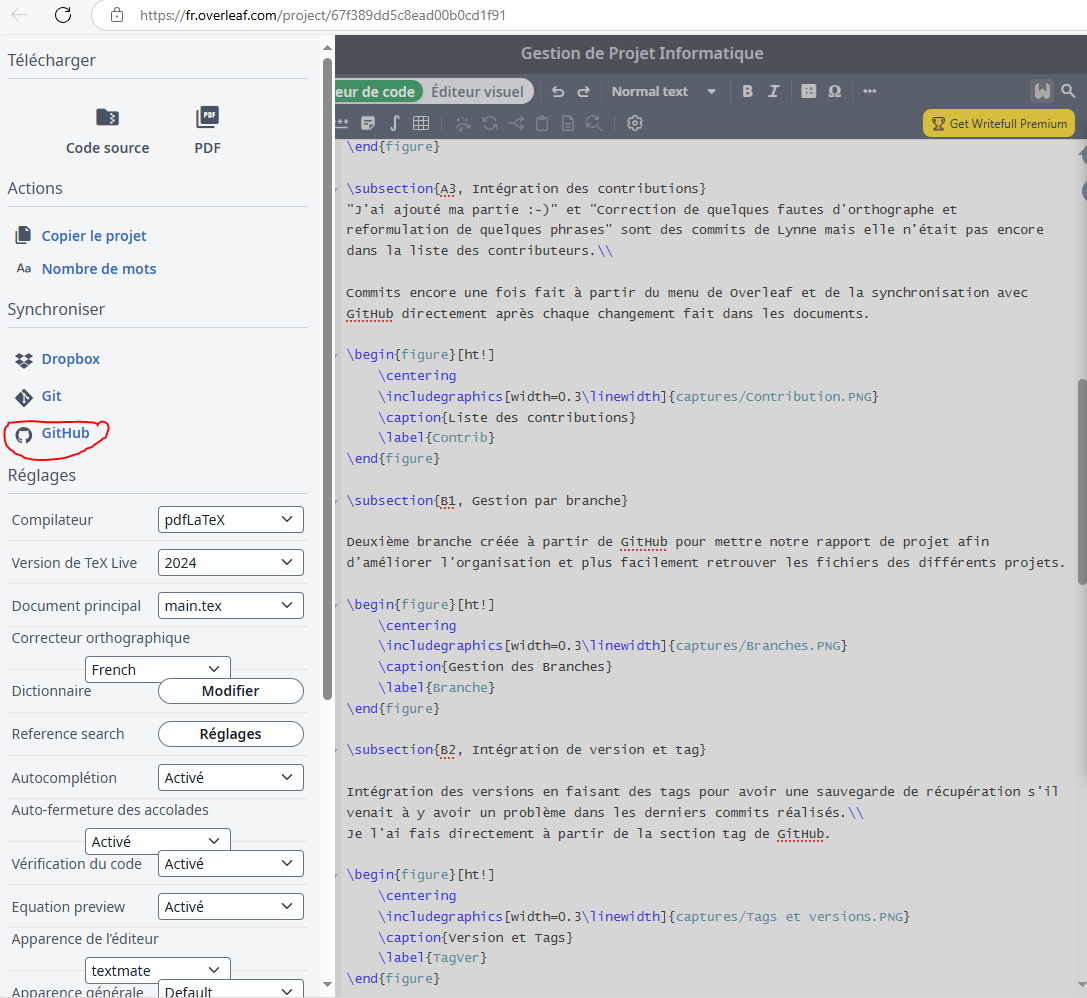
\includegraphics[width=0.5\linewidth]{captures/Synchroniser avec GitHub_1.PNG}
    \caption{Synchronisation avec GitHub}
    \label{Synch1}
\end{figure}

\begin{figure}[H]
    \centering
    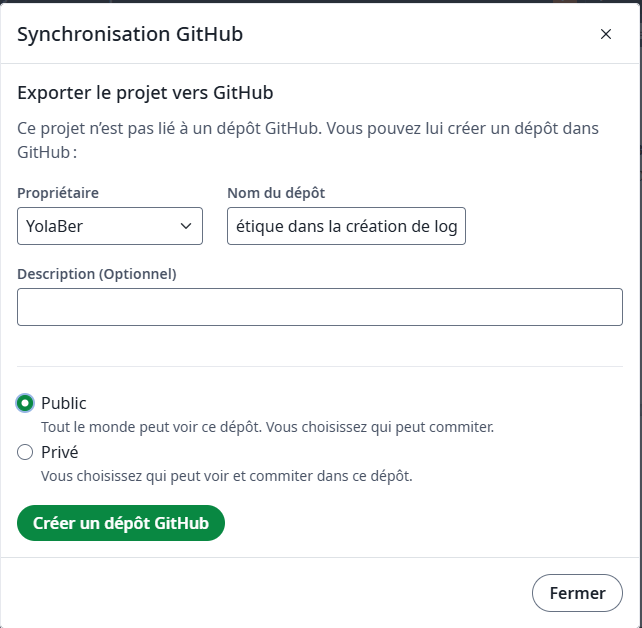
\includegraphics[width=0.5\linewidth]{captures/Synchroniser avec GitHub_2.PNG}
    \caption{Comment synchroniser son projet avec GitHub (partie 2)}
    \label{synch2}
\end{figure}

\begin{figure}[H]
    \centering
    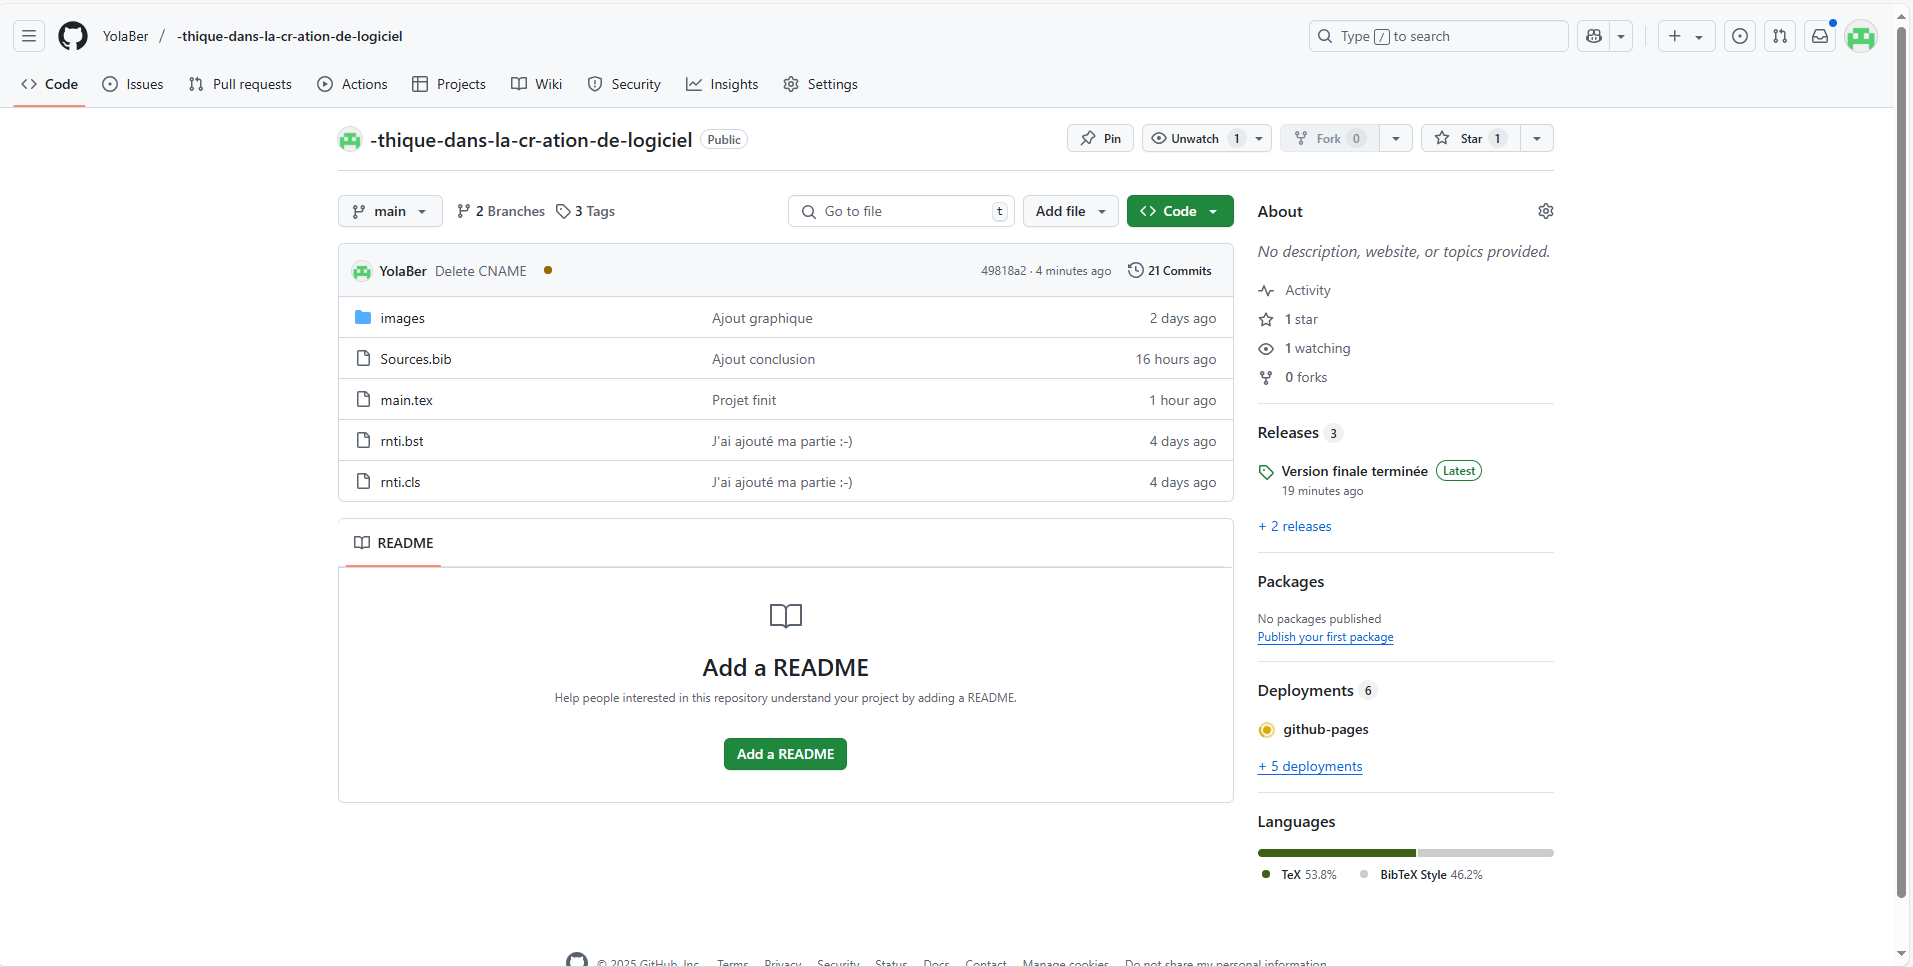
\includegraphics[width=0.5\linewidth]{captures/DPTGIT.PNG}
    \caption{Dépôt GitHub}
    \label{DPTGit}
\end{figure}

\subsection{A3, Intégration des contributions}
"J'ai ajouté ma partie :-)" et "Correction de quelques fautes d'orthographe et reformulation de quelques phrases" sont des commits de Lynne mais elle n'était pas encore dans la liste des contributeurs.\\

Commits encore une fois fait à partir du menu de Overleaf et de la synchronisation avec GitHub directement après chaque changement fait dans les documents.

\begin{figure}[H]
    \centering
    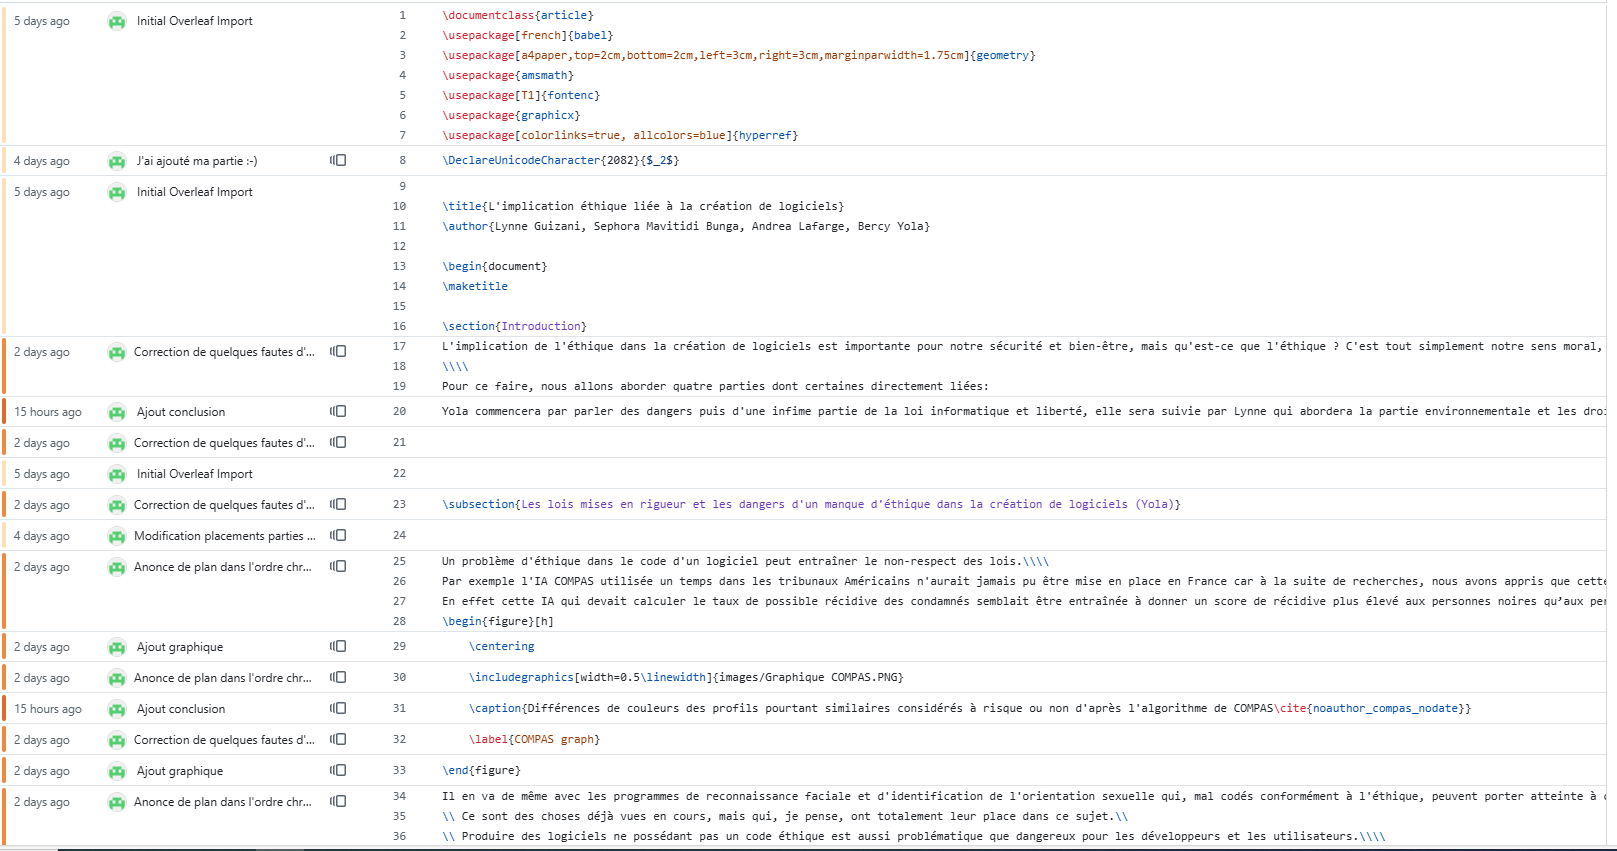
\includegraphics[width=0.5\linewidth]{captures/Contribution.PNG}
    \caption{Liste des contributions}
    \label{Contrib}
\end{figure}

\subsection{B1, Gestion par branche}

Deuxième branche créée à partir de GitHub pour mettre notre rapport de projet afin d'améliorer l'organisation et plus facilement retrouver les fichiers des différents projets.

\begin{figure}[H]
    \centering
    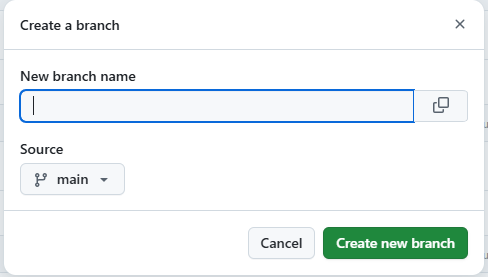
\includegraphics[width=0.5\linewidth]{captures/CB.PNG}
    \caption{Création de branche}
    \label{CB}
\end{figure}

\begin{figure}[H]
    \centering
    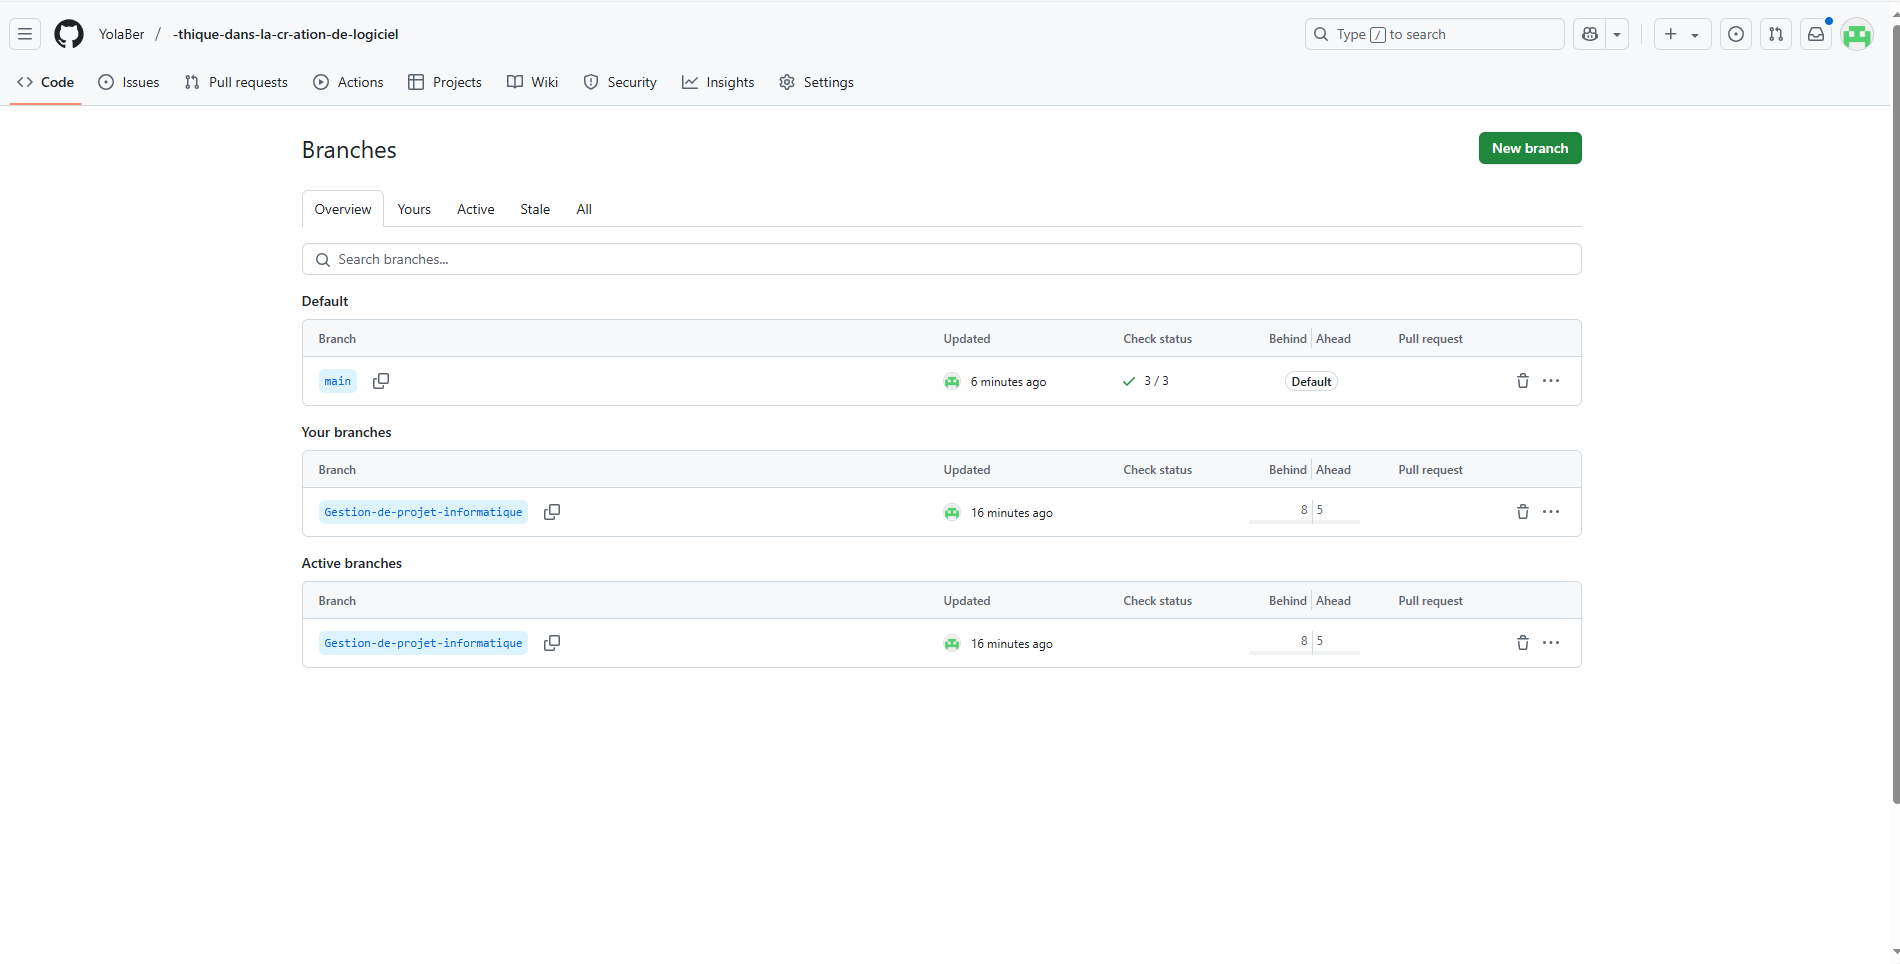
\includegraphics[width=0.5\linewidth]{captures/Branches.PNG}
    \caption{Gestion des Branches}
    \label{Branche}
\end{figure}

\subsection{B2, Intégration de version et tag}

Intégration des versions en faisant des tags pour avoir une sauvegarde de récupération s'il venait à y avoir un problème dans les derniers commits réalisés.\\
Je l'ai fait directement à partir de la section tag de GitHub.

\begin{figure}[H]
    \centering
    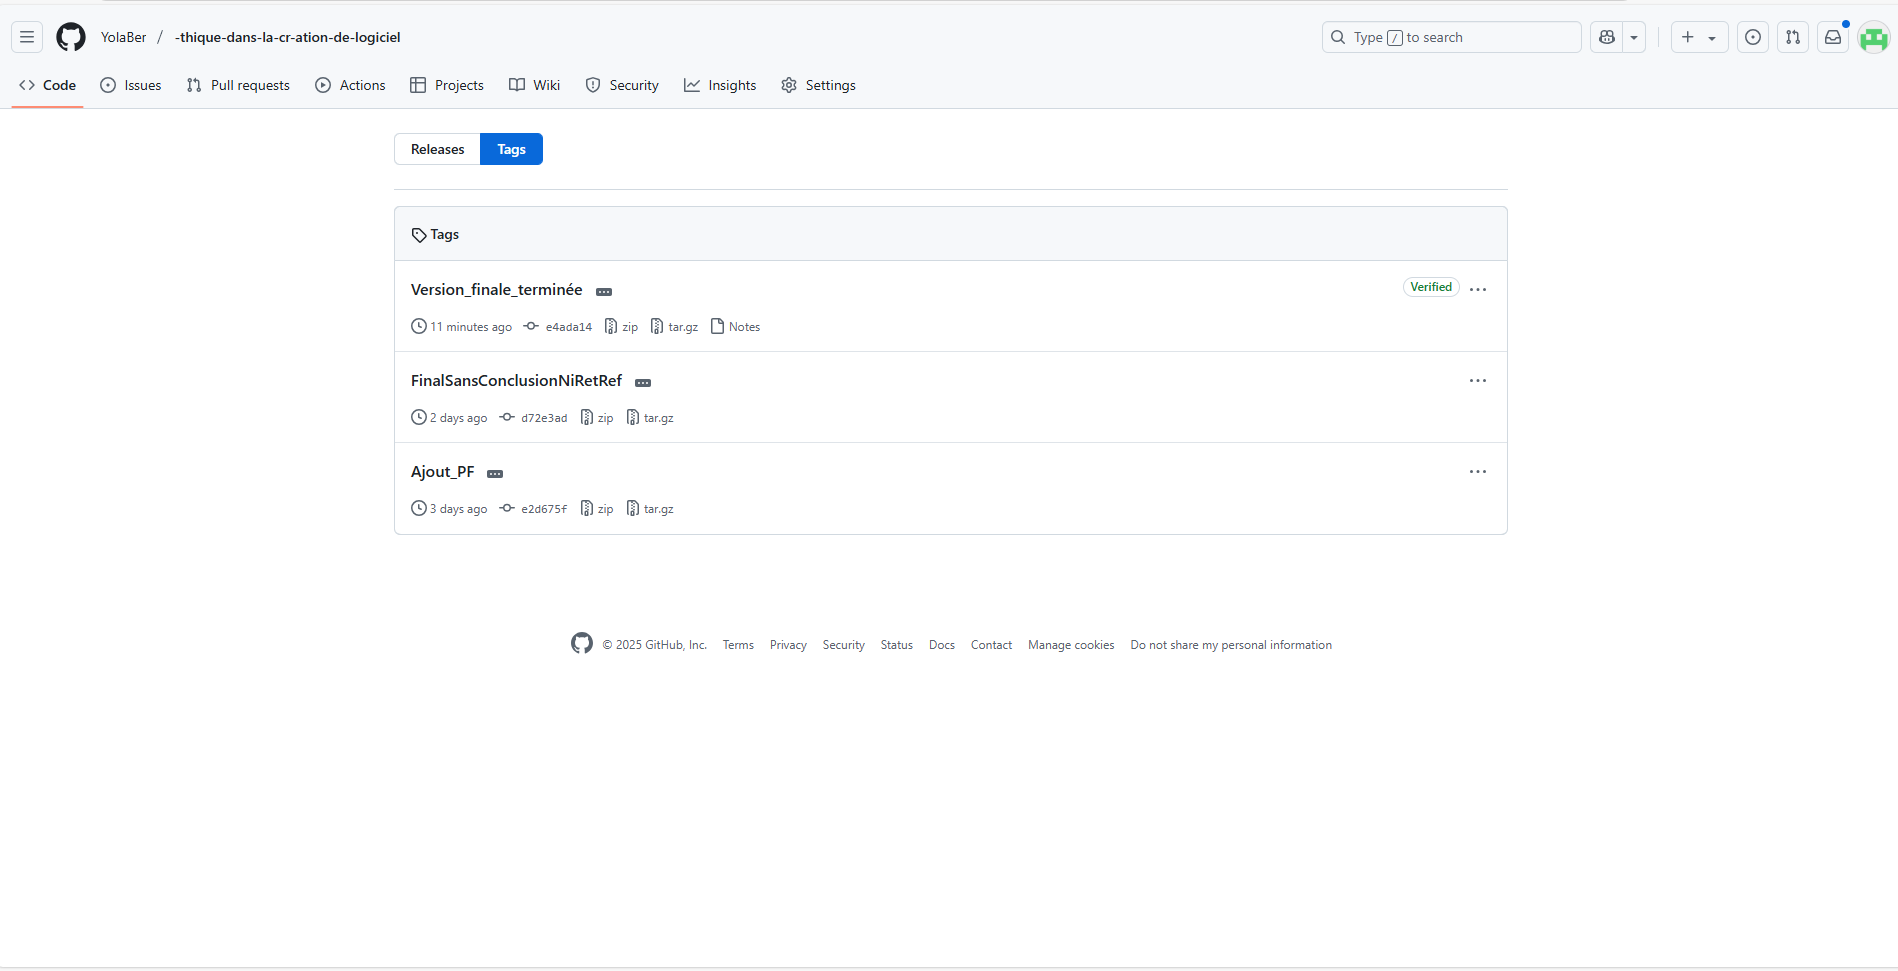
\includegraphics[width=0.5\linewidth]{captures/Tags et versions.PNG}
    \caption{Version et Tags}
    \label{TagVer}
\end{figure}

\subsection{B3, Gestion des propositions de contributions}
Un test de pull request pour insérer le rapport dans la branche dédier toujours à partir de GitHub, celui-ci est mal fait mais nous avons compris comment faire alors Andrea le refera correctement quand le rapport sera terminé. \\

\begin{figure}[H]
    \centering
    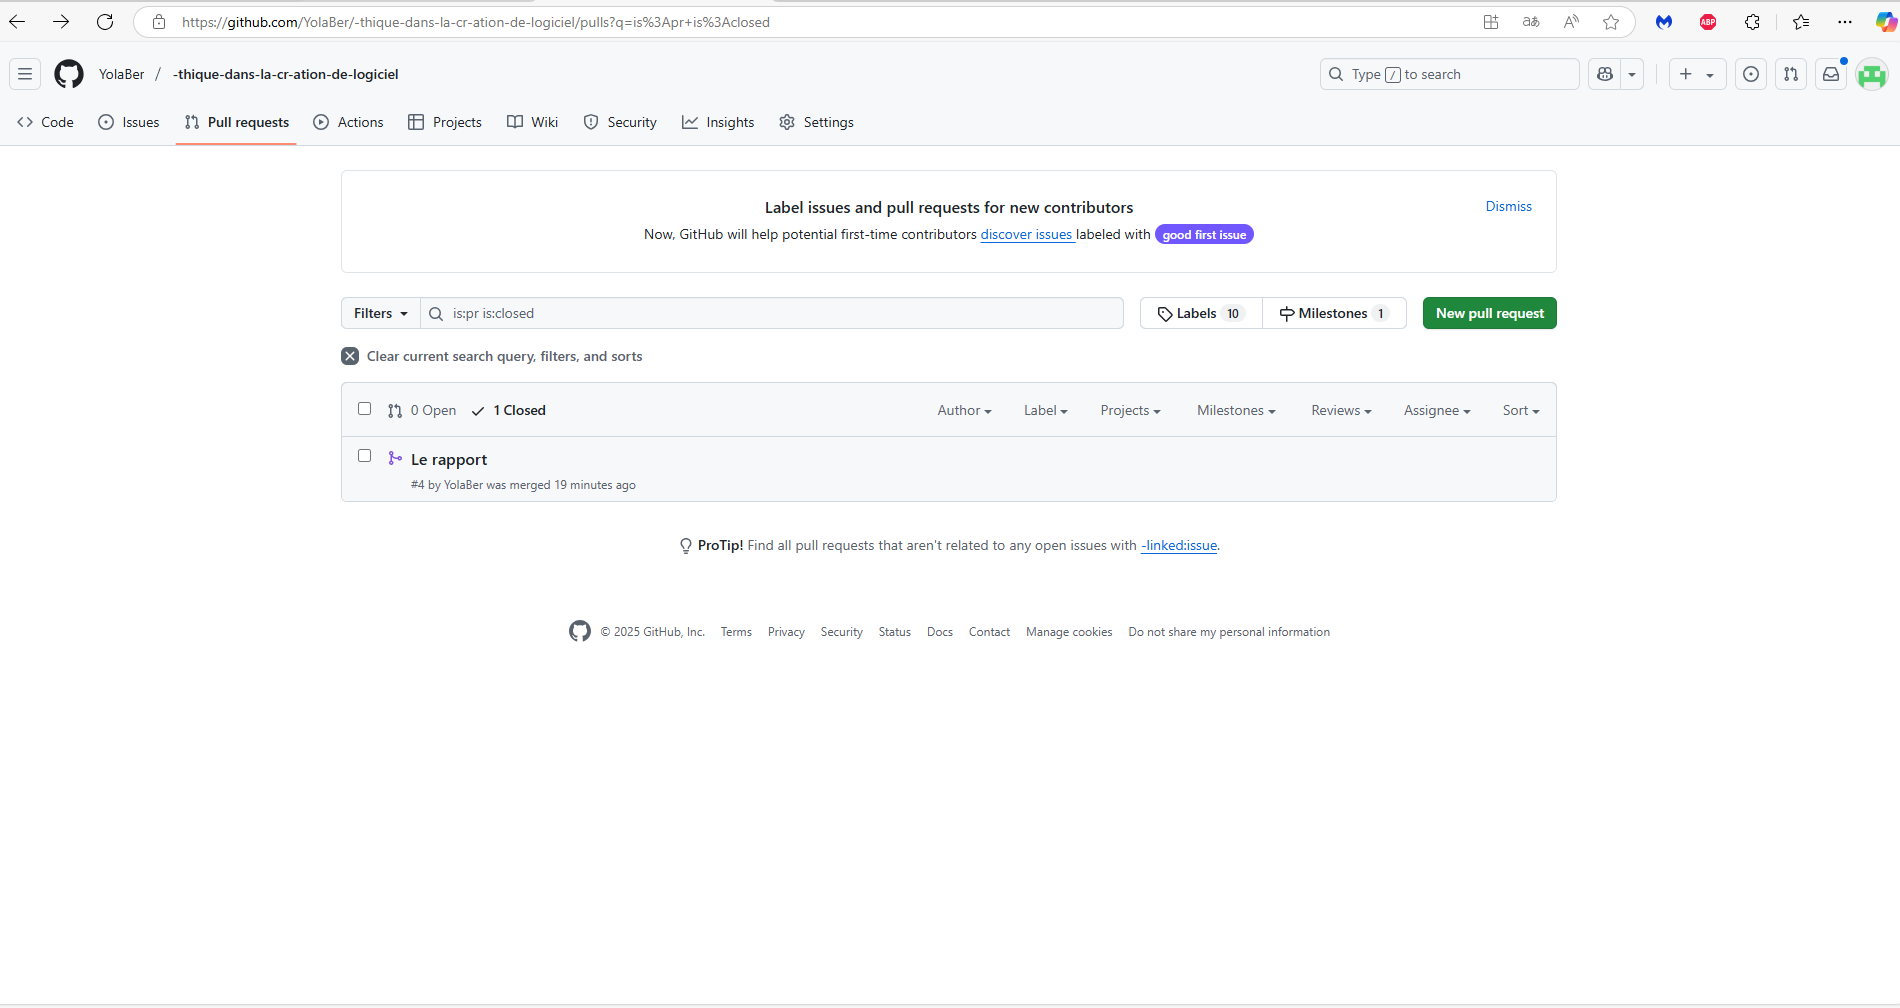
\includegraphics[width=0.5\linewidth]{captures/Pull request.PNG}
    \caption{Pull request}
    \label{Pull}
\end{figure}

\subsection{B4, Intégration de site web}
On a créé un simple site web en utilisant GitHub Pages, qui affiche le contenu du fichier index.html de la branche "Gestion-de-projet-informatique".

URL:  \url{https://yolaber.github.io/-thique-dans-la-cr-ation-de-logiciel/}

La création du site web à été fait par Lynne.

\begin{figure}[H]
    \centering
    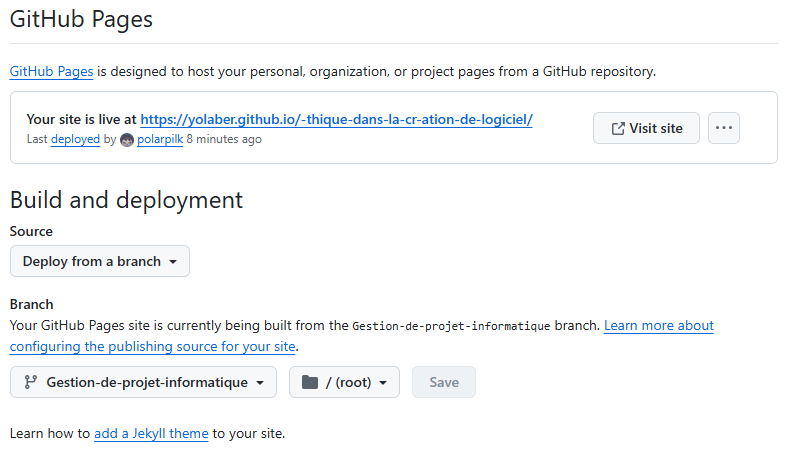
\includegraphics[width=0.5\linewidth]{captures/Site.PNG}
    \caption{Création du site web}
    \label{Créasite}
\end{figure}

\subsection{C1, Répartition des tâches et Milestone}
La répartition des tâches, c'est fait avec l'ouverture d'un Milestone et surtout les issues qu'on mettait à l'intérieur pour se tenir au courant des changement à apporter et des parties manquantes, c'était plus simple que de le dire sur un chat de groupe et attendre qu'une personne réponde car la personne avait juste à s'assigner la tâche.

\begin{figure}[H]
    \centering
    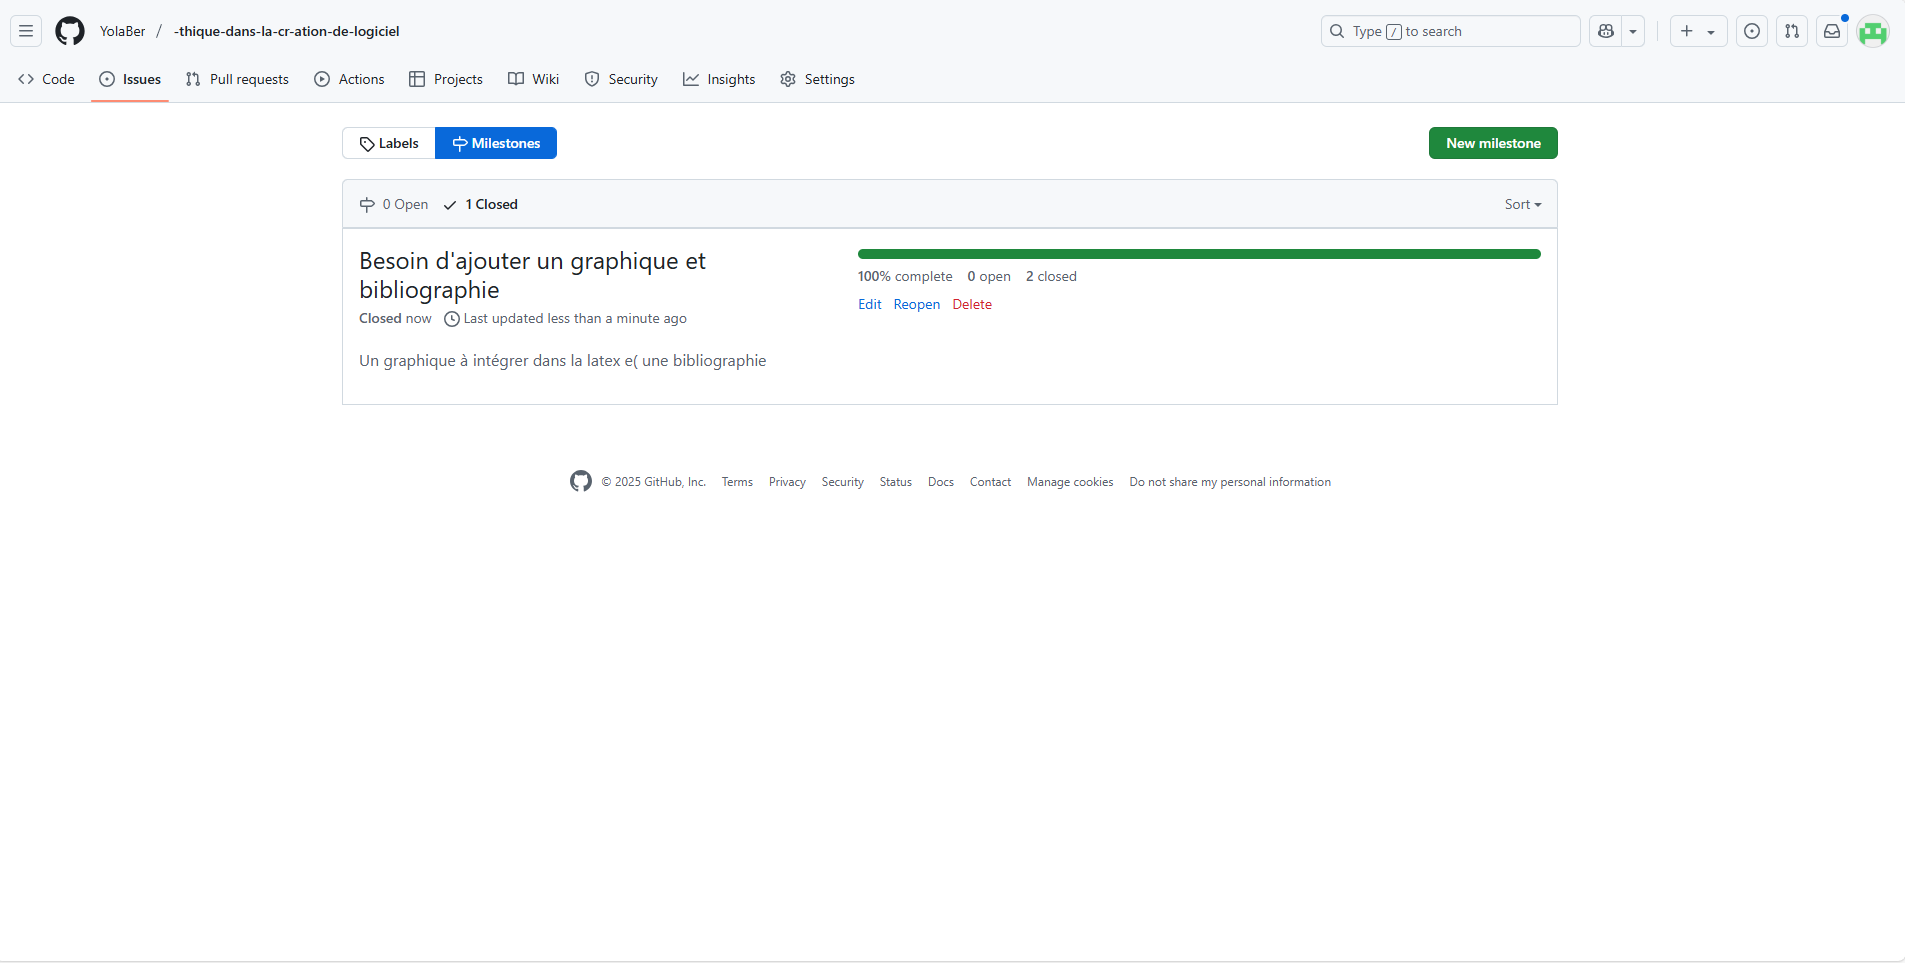
\includegraphics[width=0.5\linewidth]{captures/Milestone.PNG}
    \caption{Répartition des tâches par Milestones}
    \label{Miles}
\end{figure}

\begin{figure}[H]
    \centering
    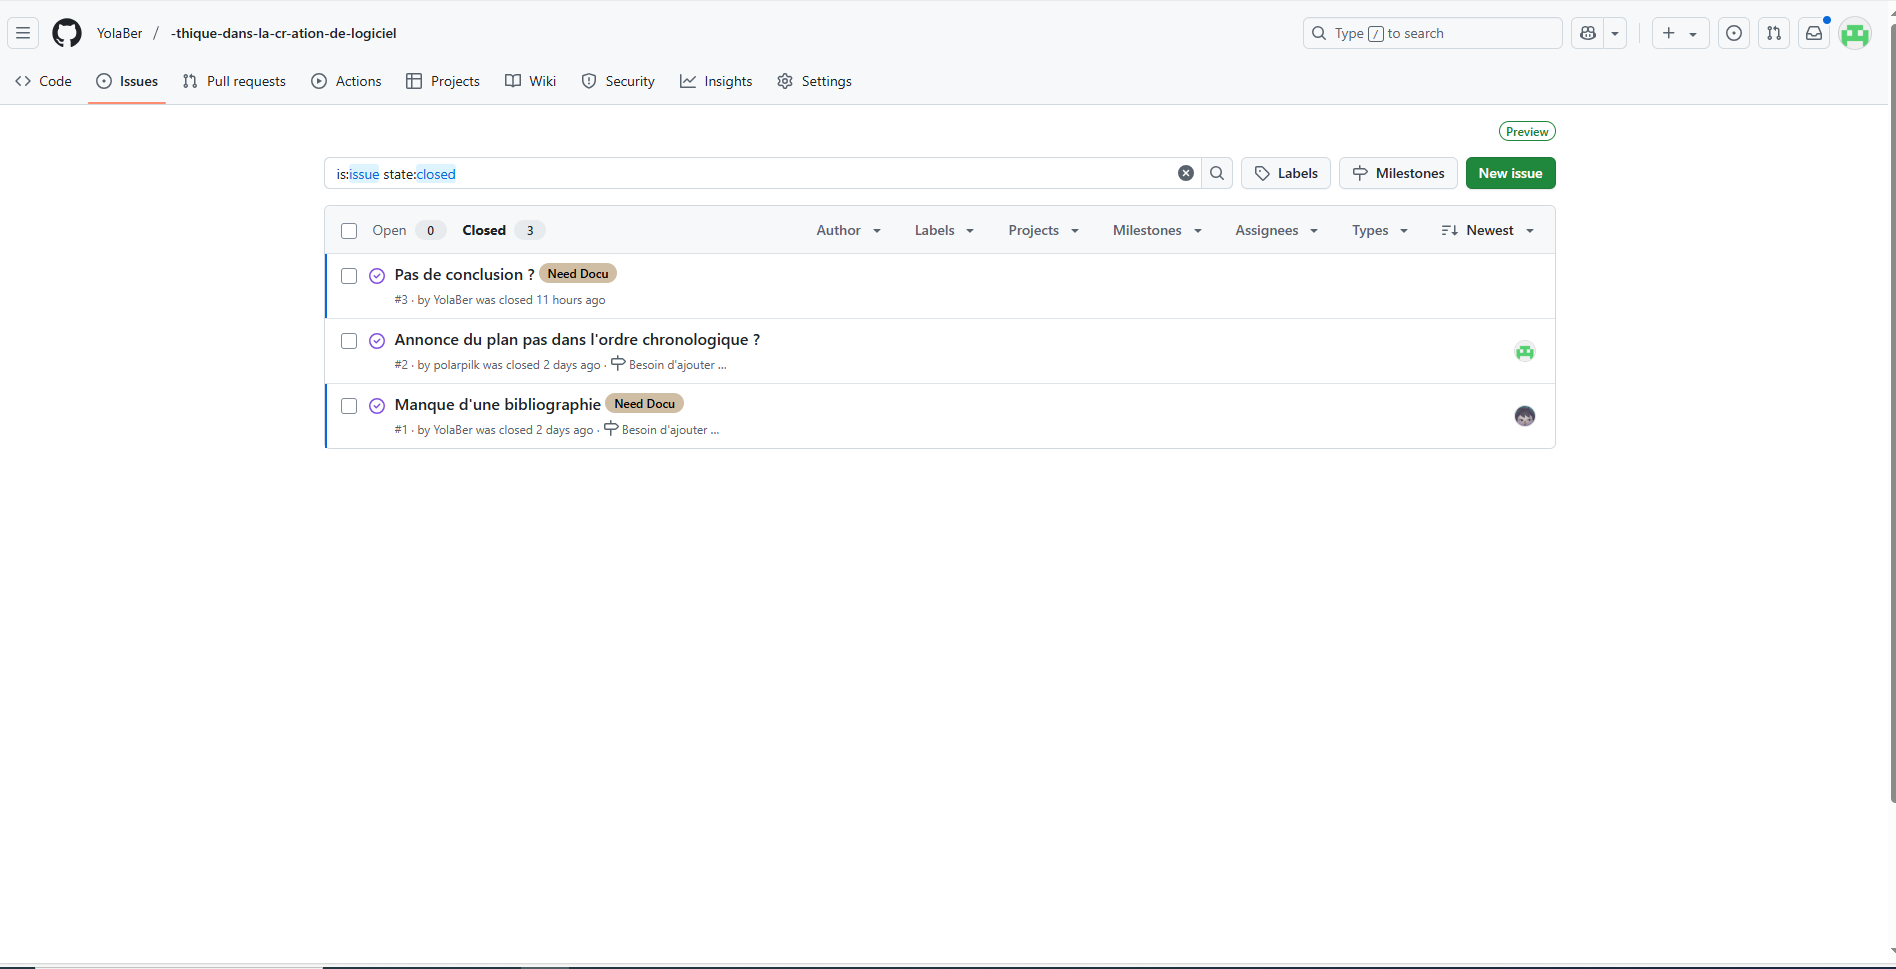
\includegraphics[width=0.5\linewidth]{captures/Issues.PNG}
    \caption{Mais aussi par Issues}
    \label{Iss}
\end{figure}

\section{Conclusion}
Ce projet nous a énormément rapporté en termes de connaissances pratiques - en effet, c'est la première fois qu'on utilise GitHub pour un projet de groupe. On a apprécié le fait qu'on peut très facilement voir les contribution de tout le monde, et le fait qu'on peut suivre les problèmes/tâches qu'on doit accomplir à l'aide de l'interface des "issues". Auparavant, on devait remonter des fils de discussion interminables pour les retrouver.  
Et maintenant, on comprend pourquoi les branches sont également indispensables : auparavant, nous copiions nos fichiers par crainte de les modifier, ce qui nous amenait à avoir 17 copies différentes du même fichier pour un seul projet. Non seulement c'est inefficace, mais cela encombrait également nos PC.
Malheureusement, on a eu du mal à bien positionner les images. On a trouvé cet aspect un peu contre-intuitif. 

\end{document}